\documentclass[11pt]{article}
\usepackage[margin=0.65in]{geometry}
\usepackage{fontspec}
\setmainfont{Helvetica Neue}
\usepackage{xcolor}
\usepackage{tikz}
\usetikzlibrary{arrows.meta,positioning,shapes.geometric,shapes.misc,fit}
\usepackage{booktabs,tabularx,array}
\usepackage{enumitem}
\usepackage{amsmath,amssymb}
\usepackage{multicol}
\usepackage{tcolorbox}
\usepackage{microtype}
\pagestyle{empty}

\definecolor{ink}{HTML}{172033}
\definecolor{muted}{HTML}{5D6678}
\definecolor{blue}{HTML}{2864DC}
\definecolor{teal}{HTML}{087E8B}
\definecolor{orange}{HTML}{D66A00}
\definecolor{paper}{HTML}{FBFCFF}
\definecolor{line}{HTML}{D8DFEB}
\definecolor{softblue}{HTML}{EDF3FF}
\definecolor{softteal}{HTML}{E8F7F7}
\definecolor{softorange}{HTML}{FFF3E5}

\color{ink}
\setlength{\parindent}{0pt}
\setlength{\parskip}{4pt}
\newcommand{\term}[1]{\textcolor{blue}{\textbf{#1}}}
\newcommand{\choice}[1]{\textcolor{teal}{\textbf{#1}}}
\newcommand{\warning}[1]{\textcolor{orange}{\textbf{#1}}}

\begin{document}

{\Huge\bfseries Probability Reasoning}\par\vspace{-2pt}
{\large A visual subway study guide for choosing distributions in ML}\par\vspace{8pt}
\textcolor{muted}{Based on \texttt{skill-probability-reasoning.md} from Phase 1, Lesson 6.}

\begin{tcolorbox}[colback=softblue,colframe=blue,boxrule=0.7pt,arc=5pt,left=9pt,right=9pt,top=7pt,bottom=7pt]
\textbf{The one job of a probability distribution:} describe what values are plausible and how likely they are. In ML, distributions describe labels, counts, measurements, noise, token choices, and uncertainty.
\end{tcolorbox}

\section*{1. Start here: identify the shape of the outcome}

\begin{center}
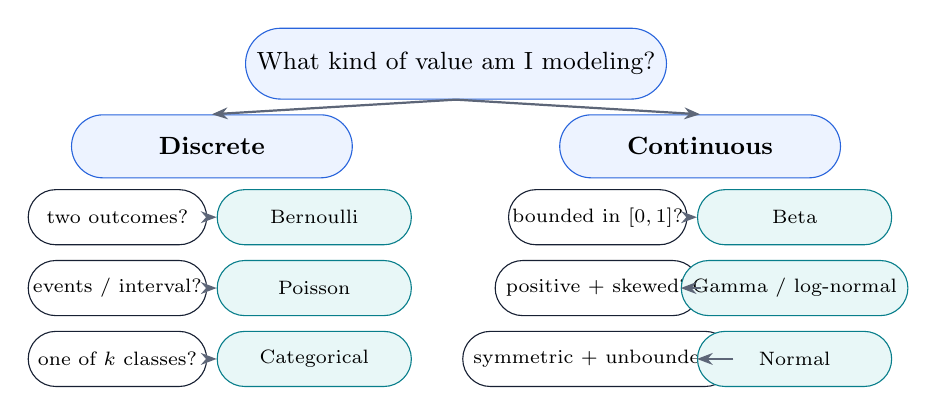
\begin{tikzpicture}[
  every node/.style={font=\small,align=center},
  start/.style={rounded rectangle,draw=blue,fill=softblue,minimum width=43mm,minimum height=9mm},
  group/.style={rounded rectangle,draw=blue,fill=softblue,minimum width=38mm,minimum height=8mm,font=\bfseries\small},
  question/.style={rounded rectangle,draw=ink,fill=white,minimum width=25mm,minimum height=7mm,font=\scriptsize},
  answer/.style={rounded rectangle,draw=teal,fill=softteal,minimum width=27mm,minimum height=7mm,font=\scriptsize},
  edge/.style={-{Stealth[length=2mm]},draw=muted,thick}
]
\node[start] (start) at (0,3.2) {What kind of value am I modeling?};
\node[group] (disc) at (-3.1,2.15) {Discrete};
\node[group] (cont) at (3.1,2.15) {Continuous};

\node[question] (two) at (-4.3,1.25) {two outcomes?};
\node[answer] (bern) at (-1.8,1.25) {Bernoulli};
\node[question] (count) at (-4.3,0.35) {events / interval?};
\node[answer] (pois) at (-1.8,0.35) {Poisson};
\node[question] (classes) at (-4.3,-0.55) {one of $k$ classes?};
\node[answer] (cat) at (-1.8,-0.55) {Categorical};

\node[question] (bounded) at (1.8,1.25) {bounded in $[0,1]$?};
\node[answer] (beta) at (4.3,1.25) {Beta};
\node[question] (skewed) at (1.8,0.35) {positive + skewed?};
\node[answer] (gamma) at (4.3,0.35) {Gamma / log-normal};
\node[question] (symmetric) at (1.8,-0.55) {symmetric + unbounded?};
\node[answer] (normal) at (4.3,-0.55) {Normal};

\draw[edge] (start.south) -- (disc.north);
\draw[edge] (start.south) -- (cont.north);
\foreach \q/\a in {two/bern,count/pois,classes/cat,bounded/beta,skewed/gamma,symmetric/normal}
  \draw[edge] (\q.east) -- (\a.west);
\end{tikzpicture}
\end{center}

\textbf{Decision checklist — ask these six questions before choosing:} discrete or continuous? bounded or unbounded? two outcomes or many? symmetric or skewed? independent or correlated? rate, count, proportion, or measurement?

\subsection*{Complete decision tree: every branch from the source guide}
\small
\renewcommand{\arraystretch}{1.2}
\begin{tabularx}{\textwidth}{>{\raggedright\arraybackslash}p{0.22\textwidth} >{\raggedright\arraybackslash}p{0.30\textwidth} X}
\toprule
\textbf{Value type} & \textbf{Question} & \textbf{Choose} \\
\midrule
Discrete & Two outcomes & Bernoulli $(p)$ \\
Discrete & $k$ outcomes, one trial & Categorical $(p_1,\ldots,p_k)$ \\
Discrete & $k$ outcomes, $n$ trials & Multinomial $(n,p_1,\ldots,p_k)$ \\
Discrete & Successes in $n$ trials & Binomial $(n,p)$ \\
Discrete & Events per interval & Poisson $(\lambda)$ \\
Discrete & Trials until first success & Geometric $(p)$ \\
Discrete & Trials until $r$ successes & Negative Binomial $(r,p)$ \\
Continuous & Symmetric and bell-shaped & Normal $(\mu,\sigma)$ \\
Continuous & Positive and right-skewed & Log-normal or Exponential \\
Continuous & Bounded in $[0,1]$ & Beta $(\alpha,\beta)$ \\
Continuous & Positive with flexible shape & Gamma $(\alpha,\beta)$ \\
Continuous & Time between events & Exponential $(\lambda)$ \\
Continuous & Heavy tails / outliers & Student's $t$ $(\nu)$ or Cauchy \\
Continuous & Multivariate, bell-shaped & Multivariate Normal \\
Continuous & Values sum to 1 (a simplex) & Dirichlet $(\alpha)$ \\
\bottomrule
\end{tabularx}
\normalsize

\section*{2. Discrete vs. continuous: the most important split}

\begin{center}
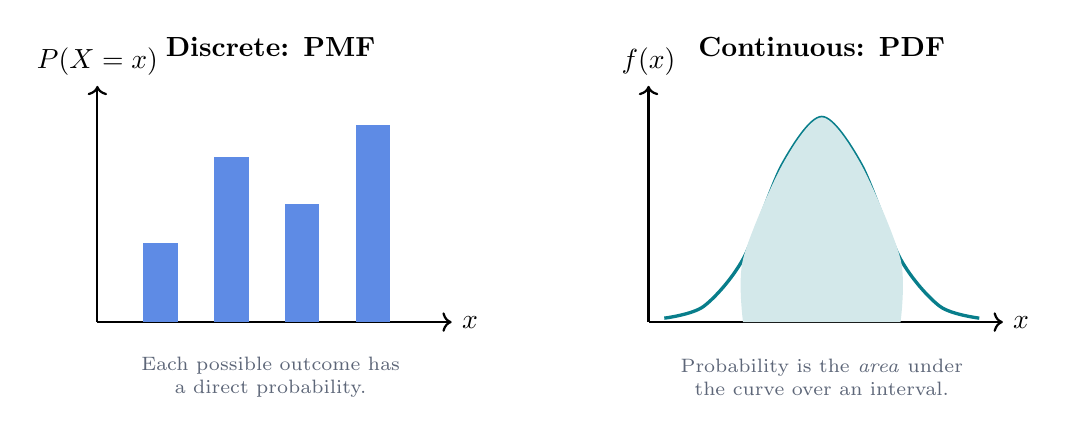
\begin{tikzpicture}[x=1cm,y=1cm]
  \node[font=\bfseries] at (2.2,3.5) {Discrete: PMF};
  \draw[->,thick] (0,0) -- (4.5,0) node[right] {$x$};
  \draw[->,thick] (0,0) -- (0,3) node[above] {$P(X=x)$};
  \foreach \x/\h in {0.8/1.0,1.7/2.1,2.6/1.5,3.5/2.5}{
    \fill[blue!75] (\x-0.22,0) rectangle (\x+0.22,\h);
  }
  \node[font=\scriptsize,text=muted,align=center] at (2.2,-0.7) {Each possible outcome has\\a direct probability.};

  \begin{scope}[xshift=7cm]
    \node[font=\bfseries] at (2.2,3.5) {Continuous: PDF};
    \draw[->,thick] (0,0) -- (4.5,0) node[right] {$x$};
    \draw[->,thick] (0,0) -- (0,3) node[above] {$f(x)$};
    \draw[teal,very thick,smooth] plot coordinates {(0.2,0.05) (0.7,0.2) (1.2,0.8) (1.7,2.0) (2.2,2.6) (2.7,2.0) (3.2,0.8) (3.7,0.2) (4.2,0.05)};
    \fill[teal!18] plot[smooth] coordinates {(1.2,0) (1.2,0.8) (1.7,2.0) (2.2,2.6) (2.7,2.0) (3.2,0.8) (3.2,0)} -- cycle;
    \node[font=\scriptsize,text=muted,align=center] at (2.2,-0.7) {Probability is the \emph{area} under\\the curve over an interval.};
  \end{scope}
\end{tikzpicture}
\end{center}

\begin{tcolorbox}[colback=softorange,colframe=orange,boxrule=0.7pt,arc=5pt,left=9pt,right=9pt,top=6pt,bottom=6pt]
\warning{Common trap:} a PDF height is not a probability. A PDF can be greater than 1; only its total area must equal 1. Classification uses a discrete PMF. Continuous latent variables and measurement noise use PDFs.
\end{tcolorbox}

\section*{3. Fast map: common ML situations}

\renewcommand{\arraystretch}{1.35}
\begin{tabularx}{\textwidth}{>{\raggedright\arraybackslash}p{0.31\textwidth} >{\raggedright\arraybackslash}p{0.25\textwidth} X}
\toprule
\textbf{Situation} & \textbf{Distribution} & \textbf{Why} \\
\midrule
Binary classifier: spam / not spam & Bernoulli & Exactly two outcomes; probability often comes from sigmoid. \\
Multi-class classifier & Categorical & One class out of $k$; probabilities come from softmax and sum to 1. \\
Next-token prediction & Categorical over vocabulary & The model chooses one token from many possible tokens. \\
Normalized pixel intensity & Beta or Uniform $[0,1]$ & The value is bounded; choose from the observed image statistics. \\
Number of events in a time window & Poisson & Counts events per interval; assumes mean = variance. \\
Time until the next event & Exponential & Models waiting time for a constant event rate. \\
Measurement error / regression noise & Normal & Symmetric, unbounded deviations around a mean. \\
A percentage or probability & Beta & Values stay inside $[0,1]$. \\
Positive, skewed duration or price & Gamma / log-normal & Never negative and usually has a long right tail. \\
VAE latent prior & Standard Normal & Simple continuous prior: $\mu=0$, $\sigma=1$. \\
Bayesian prior on a proportion & Beta & $\alpha$ and $\beta$ represent the prior belief. \\
Bayesian prior on category weights & Dirichlet & An $\alpha$ vector is a prior over categorical probabilities. \\
Outlier-robust regression & Student's $t$ & Low degrees of freedom gives heavier tails than a normal. \\
Duration / lifetime modeling & Weibull or Gamma & Shape and scale model positive durations. \\
Topic distribution per document (LDA) & Dirichlet & $\alpha<1$ encourages sparse topic mixtures. \\
\bottomrule
\end{tabularx}

\section*{4. When distributions go wrong}

\begin{enumerate}[leftmargin=18pt,itemsep=4pt]
  \item \warning{Normal for a nonnegative quantity:} normal distributions allow negative prices and distances. Consider gamma or log-normal instead.
  \item \warning{Bernoulli for multi-class labels:} Bernoulli is binary. A one-of-$k$ label needs categorical probabilities.
  \item \warning{Poisson with very different mean and variance:} Poisson assumes they are equal. If variance is larger, consider negative binomial.
  \item \warning{Treating correlated observations as independent:} time-series, spatial, and grouped data violate independence. Use autoregressive or hierarchical models.
\end{enumerate}

\section*{5. Common mistakes}

\begin{enumerate}[leftmargin=18pt,itemsep=4pt]
  \item \warning{Confusing a PDF value with a probability:} a PDF can exceed 1. Probability is the area found by integrating over an interval.
  \item \warning{Forgetting what softmax means:} softmax outputs categorical probabilities, not independent Bernoulli probabilities. Its outputs sum to 1 by construction.
  \item \warning{Using a uniform prior despite domain knowledge:} an informative prior can reduce variance without biasing the result when it is chosen well.
  \item \warning{Treating log-probabilities as probabilities:} log-probabilities do not sum to 1; they are usually negative or zero.
\end{enumerate}

\section*{6. Quick reference: distribution properties}

\small
\renewcommand{\arraystretch}{1.18}
\begin{tabularx}{\textwidth}{>{\raggedright\arraybackslash}p{0.20\textwidth} >{\raggedright\arraybackslash}p{0.14\textwidth} >{\raggedright\arraybackslash}p{0.34\textwidth} X}
\toprule
\textbf{Distribution} & \textbf{Support} & \textbf{Mean and variance} & \textbf{Key property} \\
\midrule
Bernoulli$(p)$ & $\{0,1\}$ & Mean $p$; variance $p(1-p)$ & Simplest discrete distribution \\
Binomial$(n,p)$ & $\{0,\ldots,n\}$ & Mean $np$; variance $np(1-p)$ & Sum of $n$ Bernoulli trials \\
Poisson$(\lambda)$ & $\{0,1,2,\ldots\}$ & Mean $\lambda$; variance $\lambda$ & Mean equals variance \\
Normal$(\mu,\sigma^2)$ & $(-\infty,\infty)$ & Mean $\mu$; variance $\sigma^2$ & Maximum entropy for fixed mean/variance \\
Exponential$(\lambda)$ & $[0,\infty)$ & Mean $1/\lambda$; variance $1/\lambda^2$ & Memoryless \\
Beta$(\alpha,\beta)$ & $[0,1]$ & Mean $\alpha/(\alpha+\beta)$; variance $\alpha\beta/((\alpha+\beta)^2(\alpha+\beta+1))$ & Conjugate to Binomial \\
Gamma$(\alpha,\beta)$ & $(0,\infty)$ & Mean $\alpha/\beta$; variance $\alpha/\beta^2$ & Conjugate to Poisson \\
Dirichlet$(\alpha)$ & Simplex & Mean $\alpha_i/\sum_j\alpha_j$; variance: see formula & Conjugate to Categorical \\
\bottomrule
\end{tabularx}
\normalsize

\begin{tcolorbox}[colback=softteal,colframe=teal,boxrule=0.7pt,arc=5pt,left=9pt,right=9pt,top=6pt,bottom=6pt]
\textbf{One-sentence memory aid:} Choose the distribution whose allowed values and shape match the thing you are modeling—then verify its assumptions before trusting its results.
\end{tcolorbox}

\vfill
\small\textcolor{muted}{Source: \texttt{skill-probability-reasoning.md} — Phase 1, Lesson 6.}
\end{document}
